\chapter{Introduction}
\label{CHAP:intro}

The focus of this dissertation of is on using simulation studies to assess the impact of treatment switching on the analysis of overall survival in clinical trials for oncology when progression free survival and overall survival are correlated. In this chapter I briefly outline the design of a typical Oncology Clinical Trial, the problem of treatment switching and the evidence for correlation between endpoints. In Chapter \ref{CHAP:methods} I review some methods to address this problem and outline some open questions in their implementation. The bulk of this dissertation is then concerned with the design and results of my new simulation studies as described in Chapter \ref{C:chap_sim2} and Chapter \ref{C:chap_sim3}. 

\section{Phase III Oncology Clinical Trials Design}

\subsection{Design}
To summarise the designs and endpoints used in oncology Phase III clincial trials I refer to \cite{DesignOnco2013}, a critical review of oncology trial designs.
\begin{quote}
Phase III oncology trials are typically double-blinded and randomized trials. Stratification techniques may be used to ensure a balanced distribution of specific important patient baseline characteristics among the treatment arms to control for confounding. In the two arm parallel arm design, patients
are randomized to either the study drug or the standard of care.
\end{quote}
While \cite{DesignOnco2013} further note that ``Seamless Phase II/III trials are now commonly being explored'' for the purposes of this report I will only consider standard two arm parallel designs and for clarity will use experimental therapy to refer to the study drug and control therapy to refer to standard of care. 

\subsection{Endpoints}

\cite{DesignOnco2013} define the main efficacy outcomes examined in Phase III oncology clinical trials as follows where PD refers to progression of disease commonly defined using RECIST criteria \citep{RECIST11}. Without going into detail progression of disease indicates an increase in tumor size from baseline.

\begin{itemize}
\item ``Overall survival (OS) is defined as the time from randomization until death from any cause, and is an endpoint that is most commonly used in Phase III oncology trials.''
\item ``Progression free survival (PFS) is defined as the time from randomization until PD or death, and is a common endpoint for Phase III oncology trials. While PFS may result in regulatory registration, it is often an ``accelerated'' approval to be followed by sufficient evidence from OS for ``full'' approval. PFS is commonly used as a surrogate for OS and OS is generally considered the gold standard for approval.''
\item ``Time to progression (TTP) is defined as the time from randomization until PD (death is excluded per FDA guidelines).''
\end{itemize}

It can be seen that these are all time-to-event endpoints and while there are many ways to analyse survival data I will focus on the problem of estimating a Hazard Ratio to describe the treatment effect of experimental therapy relative to control therapy. 

\section{Treatment Switching}

\cite{Latimer2014} defines treatment switching as the practice whereby ``patients randomized to the control group of a clinical trial are permitted to switch to the experimental treatment group''. They also note that the cause of this switch maybe both ethical and practical reasons. Following their terminology I will use the term treatment switching rather than crossover to avoid any confusion with crossover clinical trials such as those commonly used to estimate pharmacokinetics. I also make a distinction between this restrictive definition of treatment switch and the practice described by \cite{DesignOnco2013} that ``Patients [in Phase III trials] are allowed for ethical reasons to take subsequent anti-cancer therapies after progressive disease on trial therapy.''. While this switch to other non experimental therapies is an important aspect of oncology trial design and many of the methods detailed in Chapter \ref{CHAP:methods} are adaptable to this situation I will not consider this further. This is primarily because such non-experimental interventions likely represent normal clinical practice and depending on the comparison of interest possibly shouldn't be adjusted for.

\subsection{Patterns of switching}

\label{S:chap_intro:pattern}
To understand the patterns of switching from control to experimental therapy a very brief review of some oncology clinical trials was made. For some studies it is clear that the decision to allow switching was made from the start of the study with a clear selection on patient eligibility, for example a requirement for patients to have documented progression before switching. Some examples for this pattern are:
\begin{itemize}

\item BREAK-3 a trial in metastatic melanoma ``Patients in the dacarbazine [control therapy] group were allowed to cross over to receive dabrafenib [experimental therapy] after progression was confirmed by independent review.'' \citep{BREAK3}

\item RECORD-1 a trial in metastatic renal cell carcinoma ``\ldots after documented progression on the basis of investigator assessment. Patients who were initially randomised to placebo [control therapy] were then able to crossover to receive open-label everolimus [experimental therapy].'' \citep{RECORD1}

\item TIVO-1 a trial in metastatic renal cell carcinoma ``Patients who had Response Evaluation Criteria in Solid Tumor (RECIST) defined disease progression, were allowed an option to cross over to tivozanib [experimental therapy] arm'' \citep{TIVO1}

\end{itemize}

For other studies the decision is made based on interim or final efficacy analysis and in this case there may be less restrictive criteria on which patients are eligible to switch:

\begin{itemize}

\item BRIM-3 a trial in metastatic melanoma ``The data and safety monitoring board determined that both the overall survival and progression-free survival end points had met the prespecified criteria for statistical significance in favor of vemurafenib [experimental therapy]. The board recommended that patients in the dacarbazine [control therapy] group be allowed to cross over to receive vemurafenib [experimental therapy]''. \citep{BRIM3}

\item COMBI-V a trial in metastatic melanoma ``the study was stopped for efficacy on July 14, 2014. A protocol amendment was issued to allow crossover to the combination-therapy [experimental therapy] group for patients assigned to the vemurafenib [control therapy] group'' \citep{COMBIV}

\end{itemize}
Finally the decision maybe made based upon evidence of efficacy seen in another trial such as:

\begin{itemize}

\item TH3RESA a trial in metastatic Breast Cancer ``\ldots after EMILIA [another trial for experimental therapy] data were reported, 13 patients who had progressive disease while receiving treatment of physician's choice [control therapy] were eligible to cross over to trastuzumab emtansine [experimental therapy] \ldots ''. \citep{TH3RESA}

\end{itemize}

These patterns of switching can be grouped as shown in Table \ref{T:chap_intro:switch}. 
\begin{table}[ht] 
\caption{Identified switching scenarios}
\centering 
\begin{tabular}{ l  l l  }
\hline
\hline

 & \multicolumn{2}{c}{When in study?}  \\
Who can                 & From  & After efficacy   \\
switch?                 & Day 1 & demonstrated     \\ 
\hline\\[0.3cm]
All patients            & n/a   &  COMBI-V \\
                        &       & BRIM-3           \\[0.3cm]
           
Patients who &  BREAK-3  & TH3RESA          \\ 
Progressed   & RECORD-1  &                   \\
             & TIVO-1    &                    \\
\hline             
\end{tabular} 
\label{T:chap_intro:switch}
\end{table}

\subsection{What is the impact on analysis}

Depending on the pattern of switching the impact of switch on the endpoints of PFS and OS will be varied. By considering again Table \ref{T:chap_intro:switch} it is clear that for trials where switching is restricted to patients who have progressed there will be minimal impact on analysis of PFS (ignoring the operational complexity of investigator vs independent assessment). For trials where the decision to switch is based on demonstration of efficacy with the trial then there will be no impact on those endpoints at the time of initial analysis. However, with oncology trials it is common to perform additional analysis at later time points with more mature data which could be affected for all endpoints. An example of this is shown in Table \ref{T:chap_intro:BRIM3} comparing the results of BRIM-3 as initally reported by \cite{BRIM3} with the updated report of \cite{BRIM3UPDATE}. From these it can be seen that the amount of switching increases but also so does the maturity of the data (considering the number of events observed). It can also be seen the results for both progression free survival (PFS) and overall survival (OS) change, however, it is not simple to disentangle the impact of switching versus more mature data.

\begin{table}[ht] 
\caption{Results of BRIM-3}
\centering 
\begin{tabular}{ l  l l  }
\hline
\hline
                                 & Initial report      & Updated report     \\ 
                                 & \citep{BRIM3}       &  \citep{BRIM3UPDATE} \\
\hline\\[0.2cm]
Date of data cut                 & December 30, 2010   & February 1, 2012  \\[0.2cm]

Number of patients switched      & n/a                 & 83 (25\%)         \\
to experimental therapy          &                     &                    \\[0.2cm]

Deaths on control therapy        & 75 (22\%)           & 200 (59\%)        \\[0.2cm]

Progression free survival (PFS)  &  $0.26$             & $0.38$*                \\
Hazard Ratio   &  $(0.20$ to $0.33)$ & $(0.32$ to $0.46)$    \\
(95\% Confidence Interval) & & \\
\multicolumn{3}{r}{* Censoring at switch.} \\[0.2cm]

Overall survival  (OS)           &  $0.37$             & $0.76$                 \\
Hazard Ratio            &  $(0.26$ to $0.55)$ & $(0.63$ to $0.93)$     \\
(95\% Confidence Interval) & & \\
\hline
\end{tabular} 
\label{T:chap_intro:BRIM3}
\end{table}


For the case where switching only happens at progression of disease \cite{Latimer2014} and \cite{Zhang2012} show that the potential impact can be considered by partitioning overall survival time into progression free survival (PFS) and survival post progression (SPP). For each patient who receives switch treatment the survival post progression (SPP) could be extended but the progression free survival (PFS) is unmodified. This leads to a switch contaminated overall survival for the control therapy that is longer than that which would be observed in the abscence of switch. This leads to a smaller estimate of difference between control and experimental overall survival. This is illustrated in Figure \ref{F:chap_intro:pfsandpps} adapted from \cite{Latimer2014}. 

\begin{figure}[ht]
\centering
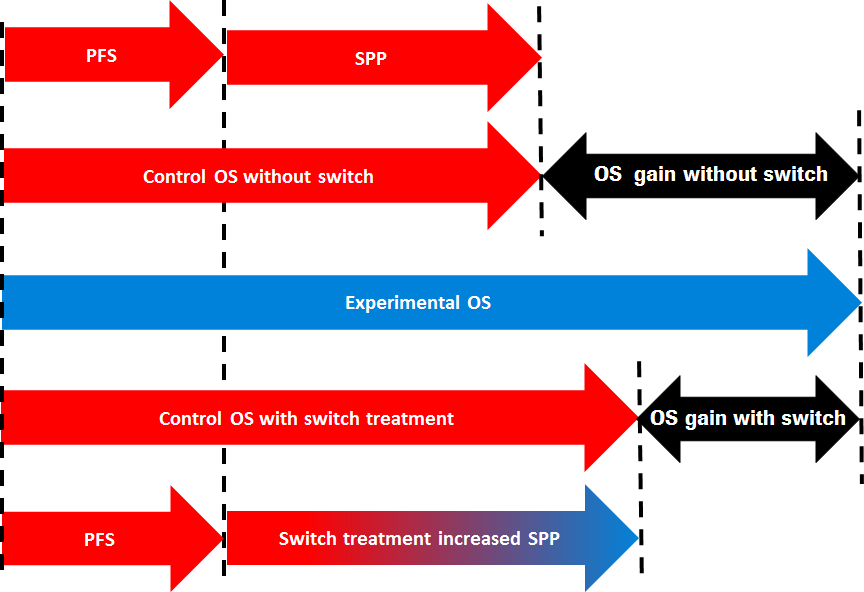
\includegraphics[width=14cm]{images/chap_intro/intro_pfsandpps.png}
\caption{\label{F:chap_intro:pfsandpps} Illustration of how treatment switching at progression can lead to contaminated estimates of overall survival. PFS = progression free survival, SPP = survival post progression, OS = overall survival. Adapted from \cite{Latimer2014}.} 
\end{figure}

\clearpage

\subsection{What is a true treatment effect?}
\label{S:chap_intro:whatest}
In this dissertation I will make commonly reference to a ``true'' or ``corrected'' treatment effect meaning the treatment effect that would have been observed if switching had not occurred. However, it will not always be the case that this ``corrected'' estimate is a useful estimate of treatment effect. For example it has been noted that if the observed treatment switch represents clinical practice no adjustment is necessarry as seen in \cite{PBAC2011} the PBAC assessment of erlotinib in Non-Small Cell Lung Cancer:
\begin{quote}
Because the EURTAC trial allowed for switching (cross-over) on disease progression, the results for overall survival inform a comparison of early versus late erlotinib; and they currently show no benefit (as at 26 January 2011 cut-off, log rank p = 0.8702).  The PBAC noted that the comparison of early versus late erlotinib is relevant in the Australian context because erlotinib is currently listed second-line in unselected patients.  Thus the clinical benefit for EGFR activating mutation positive patients of listing erlotinib as first-line treatment in addition to second-line treatment is an improvement in quality of life, but not a prolongation of life.
\end{quote}
In the event that the switch treatment does not represent clinical practice for instance if the experimental treatment is only available to both control and experimental arm patients through the clinical trial then  as noted by \cite{TSD16} ``[a comparison of randomised groups] is unlikely to be what is required [\ldots] because the ``true'' survival benefit associated with the novel intervention will be diluted due to the switching of control group patients onto the novel therapy.''  


\subsection{How does treatment switching affect interpretation?}
When considering the impact of treatment switching on the interpretation of a clinical trial it is important to consider the different questions that are being asked by stakeholders. A simplified overview of these is given below:
\begin{itemize}
\item FDA\footnote{United States Food and Drug Administration - United States Regulatory body.}, EMA\footnote{European Medicines Agency - European Regulator body.} - Benefit/Risk of an individual medicine   
\item IQWiG\footnote{Institute for Quality and Efficiency in Healthcare - Health Technology Assessment (HTA) body for Germany. } - Additional benefit compared to standard of care 
\item NICE\footnote{National Institute of Health and Care Excellence - HTA body for England and Wales.} - Additional benefit compared to standard of care extrapolated over patients life time  
\end{itemize}
In the case of considering benefit/risk of an individual medicine it is enough to show there is a treatment effect but the absolute magnitude of the effect is less important so long as it exceeds some minimum level. In this case what is important is the direction of bias with underestimation of treatment effect less concerning.

When making an assessment of benefit over standard of care it is necessary to estimate the magnitude of treatment effect with accuracy in order to enable comparisons to other therapies assuming that efficacy for these other therapies can be estimated accurately. Finally while it is not possible in this report to go into detail about methodological issues in performing an evaluation of treatment benefit extrapolated over lifetime it is sufficient to note that small changes in relative effect can translate into large differences in extrapolated absolute difference as illustrated in Figure \ref{F:chap_intro:extrapol}.

\begin{figure}[ht]
\centering
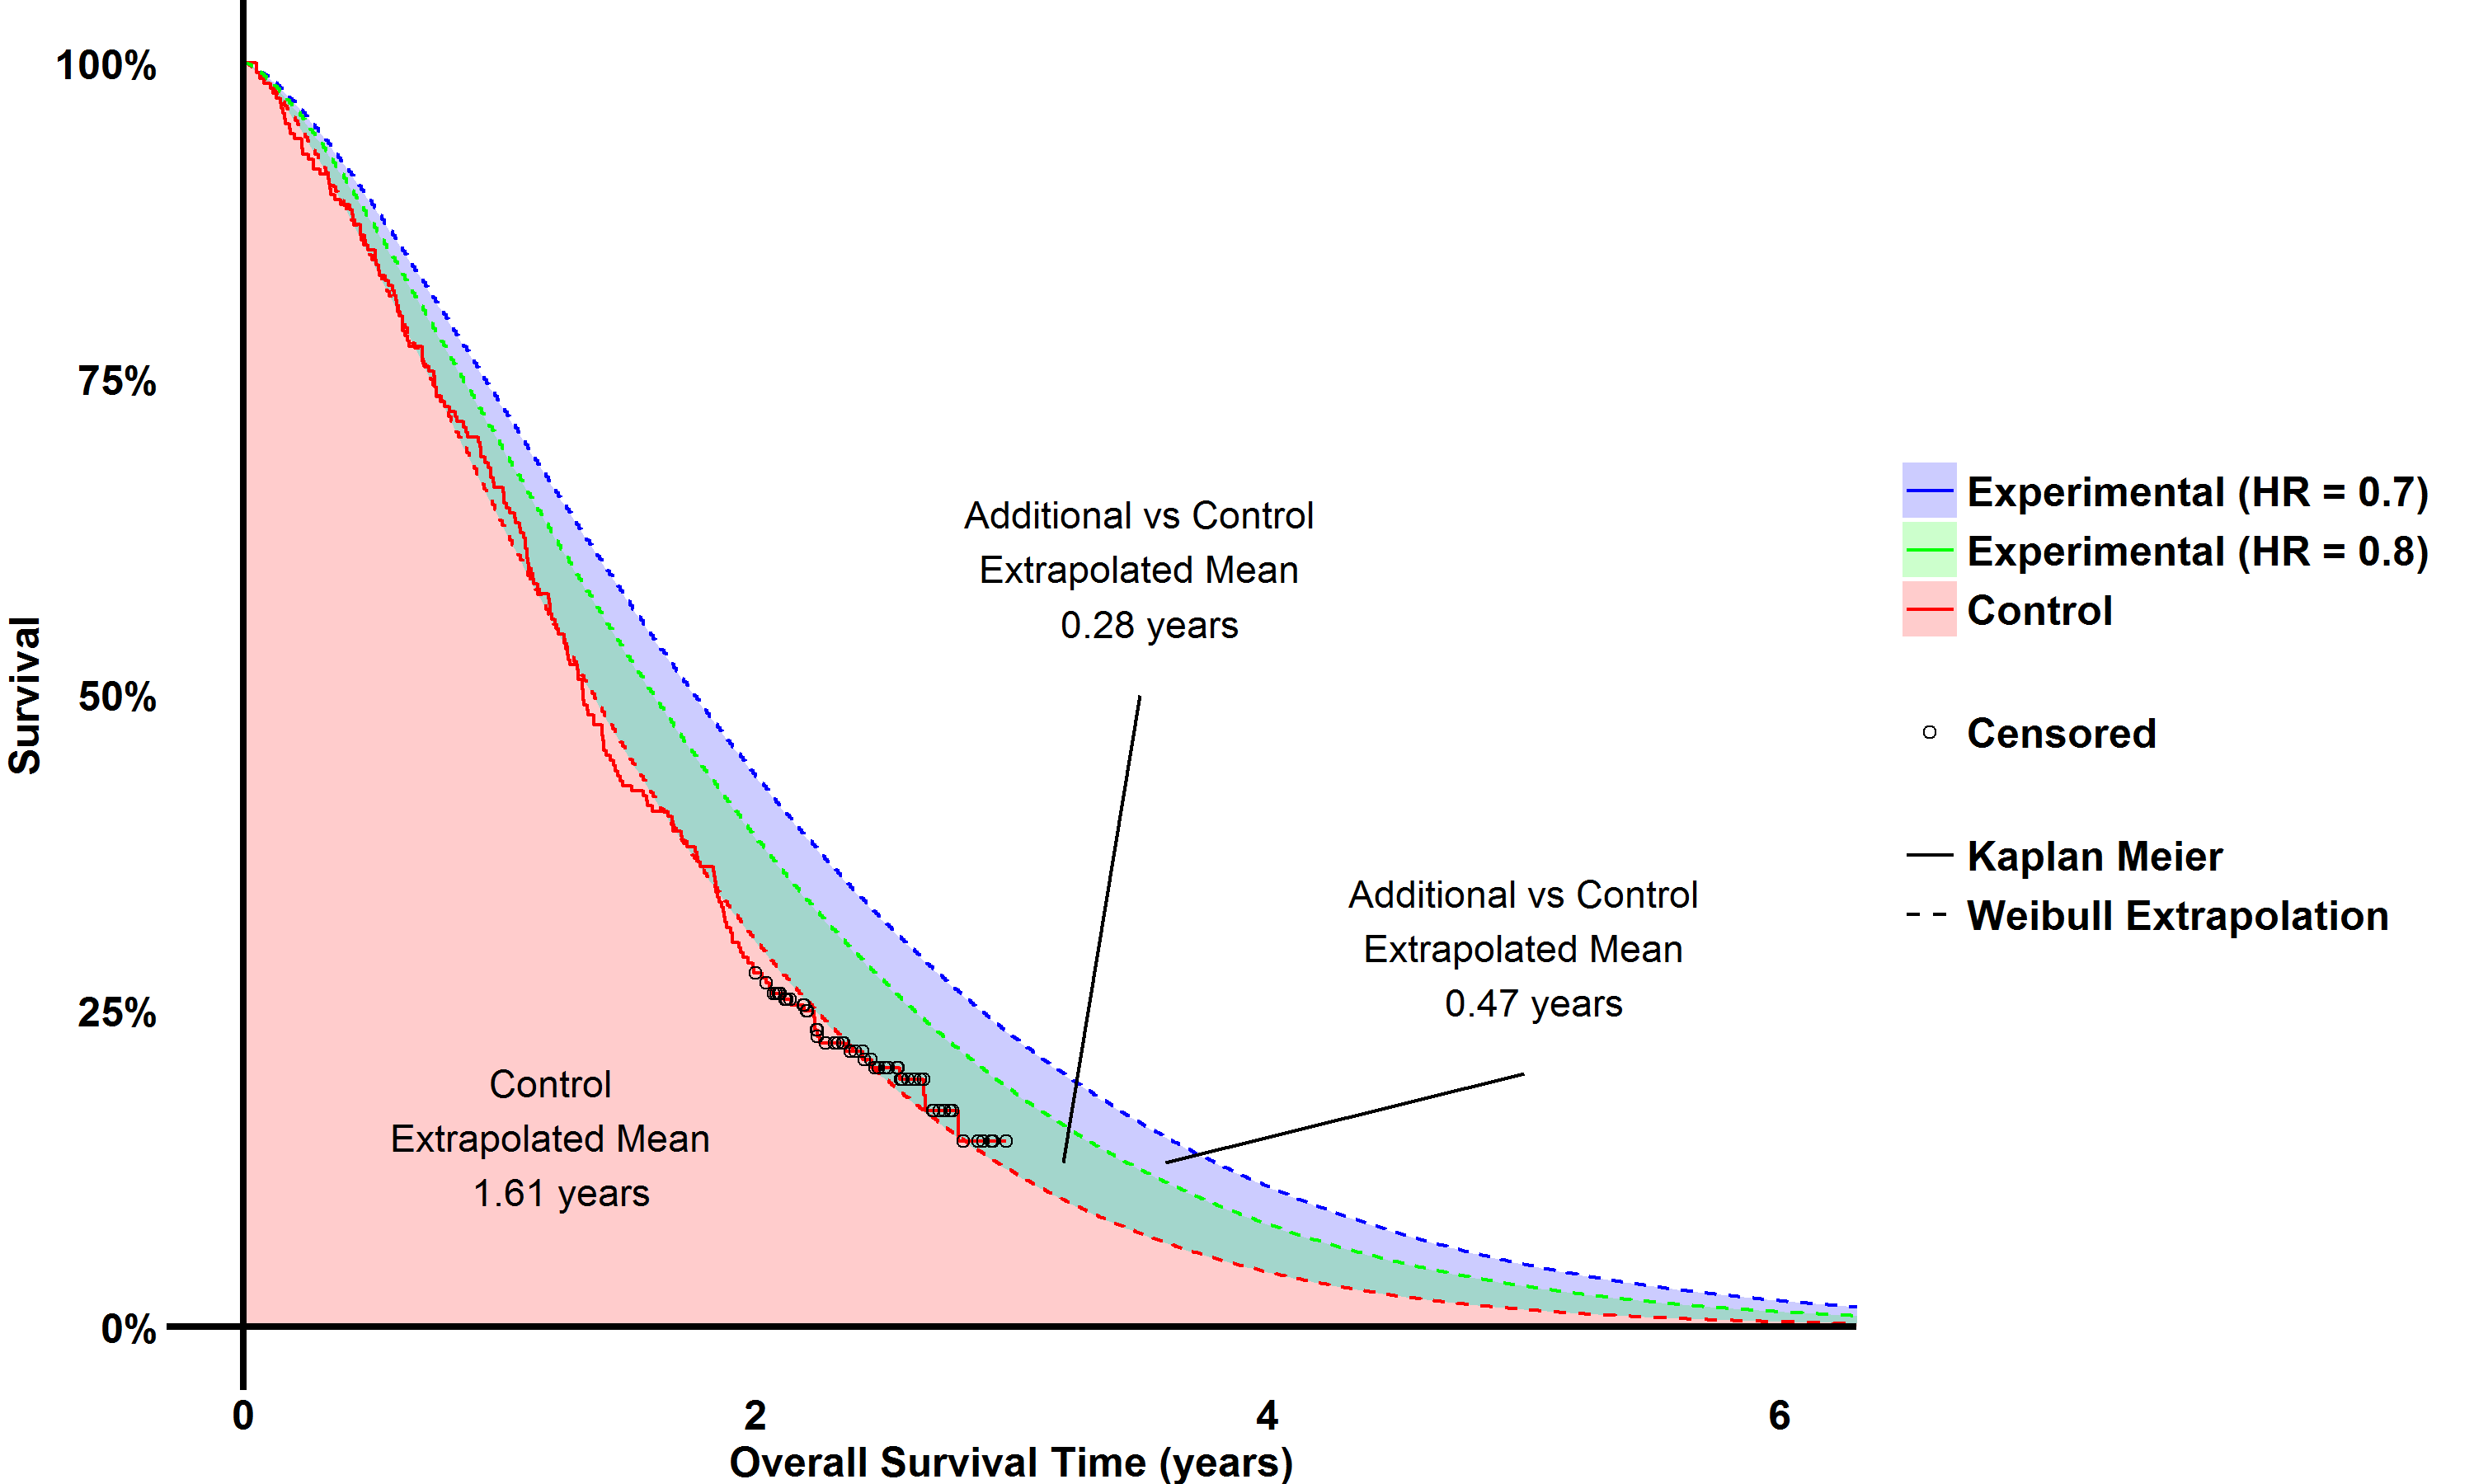
\includegraphics[width=14cm]{images/chap_intro/intro_extrapol.png}
\caption{\label{F:chap_intro:extrapol} Illustration of how quite small differences in the estimation of relative treatment effect can translate to important differences in absolute effects in the context of an economic evaluation. The mean life gain is estimated as the area under the extrapolated survival curve using the methods discussed in \cite{TSD14}.} 
\end{figure}

An additional important aspect here is to also consider the possibility of regulatory bodies accepting PFS as an endpoint to support approval of a medicine with \cite{TSD16} noting that ``showing an OS advantage may not be essential for obtaining marketing authorisation''. In these cases allowing switch at the time of progression only would not confound an analysis of PFS. However, there are clearly cases where OS benefit is required for regulatory approval such as TIVO-1 \cite{TIVO1} where there was no statistically significant difference in OS between the two arms, however, the point estimate for hazard ratio favoured the control arm:
\begin{quote}
This study met its primary end point by statistically significantly improving progression-free survival, but did impair overall survival, a secondary end point. Crossover from sorafenib to tivozanib may have confounded survival. Because of that detrimental survival, the US FDA rejected approval
\end{quote}
Though in this case it should be noted that \cite{Slaets2013} have performed simulation studies replicating this trial situation and found that it is unlikely that the absence of effect on overall survival was due to treatment switching alone.


\section{Use of simulation studies}
\label{S:chap_intro:simstudy}
In order to investigate the impact of treatment switching on the analysis of oncology trials I will use simulation studies. A simulation study is where a dataset such as a clinical trial are generated such that they have known true values for a parameter of interest to be estimated. Different statistical methods can then be used to analyse these datasets and the performance of these methods compared to the known truth. \cite{Burton2006} note that this is a common approach to assess the performance of statistical methods and advise that ``simulated data sets should have some resemblance to reality for the results to be generalizable to real situations and have any credibility''. 

In this case when considering clinical trials where multiple endpoints are measured from the same patient it is important to consider if these outcomes are correlated. In the context of treatment switching it is common for progression to be the trigger to switch from control to experimental therapy so any correlation between time to progression and overall survival could influence results. The explicit consideration of this correlation is the key difference between this work and prior simulation studies such as \cite{Morden2011}, \cite{Latimer2013} and \cite{Latimer2016}.

\subsection{Correlation between endpoints}
\label{S:chap_intro:correlation}

\cite{Ciani2014} have done a review of studies examining the correlation between progression free survival (PFS) and overall survival (OS). While this also considered studies that estimated correlations between treatment effects on these endpoints, of interest here is the correlation between PFS and OS for an individual patient. The results of the studies found that report an estimate of this correlation are reproduced in Table \ref{T:chap_intro:corr} adapted from Supplementary Table 2 of \cite{Ciani2014}. 


From Table \ref{T:chap_intro:corr} it can be seen that the estimate of correlation between PFS and OS varies both within and across different cancers. However, for the majority of the studies it is estimated to be $\ge 0.6$ and at the lowest is $0.3$ though this is for non-advanced/metastatic disease. This suggests that it is important to simulate data including correlations between these endpoints when assessing methods to adjust for overall survival. Though as will be discussed further in Section \ref{S:chap_sim_design:corr} progression free survival as a composite of time to progression and overall survival will be correlated with overall survival even if no correlation exists between time to progression and overall survival.

\begin{table}[hb] 
\caption{Reported correlations between progression free survival (PFS), time to progression (TTP) and overall survival (OS)}
\centering 
\begin{tabular}{|c|c|c|}

\multicolumn{3}{c}{Advanced Colorectal Cancer} \\
\hline
Outcome     & Estimate of Correlation    & Reference \\ 
            &  (95\% CI)    &           \\
\hline
PFS  & $R^2 = 0.61$ $(0.59 - 0.64)$  & \cite{Green2008}         \\ 
\hline
PFS  & $\rho = 0.82$ $(0.82 - 0.83)$  &  \cite{Buyse2007}       \\ 
\hline
PFS  & $\tau = 0.502$ $(0.457 - 0.548)$ &  \cite{Burzykowski2001}  (Method 1)   \\
\hline
PFS  & $\tau = 0.583$ $(0.548 - 0.619)$ &  \cite{Burzykowski2001} (Method 2) \\    
\hline    
\multicolumn{3}{c}{ } \\
\multicolumn{3}{c}{Advanced Ovarian Cancer}   \\
\hline
Outcome     & Estimate of Correlation    & Reference \\ 
            &  (95\% CI)    &           \\
\hline
 TTP  & $R^2 = 0.888$ (Not given) & \cite{Buyse2000}  \\    
\hline
PFS & $\tau = 0.857$ $(0.845 - 0.870)$ & \cite{Burzykowski2001} (Method 1)  \\    
\hline                        
PFS & $\tau = 0.839$ $(0.828 - 0.850)$ &  \cite{Burzykowski2001} (Method 2)\\        
\hline    
\multicolumn{3}{c}{ } \\
\multicolumn{3}{c}{Metastatic Breast Cancer}   \\
\hline
Outcome     & Estimate of Correlation    & Reference \\ 
            &  (95\% CI)    &           \\
\hline
PFS  & $\rho = 0.688$ $(0.686 - 0.690)$ & \cite{Burzykowski2008}   \\   
\hline     
TTP  & $\rho = 0.682$ $(0.682 - 0.684)$   & \cite{Burzykowski2008}   \\ 
\hline
\multicolumn{3}{c}{ } \\
\multicolumn{3}{c}{Progressive castrate-resistant prostate cancer }   \\
\hline
Outcome     & Estimate of Correlation    & Reference \\ 
            &  (95\% CI)    &           \\
\hline
PFS  & $\tau = 0.30$ $(0.26 - 0.32)$  & \cite{Halabi2009}   \\    
\hline
\multicolumn{3}{c}{ } \\
\multicolumn{3}{c}{Metastatic Renal Cell Carcinoma}   \\
\hline
Outcome     & Estimate of Correlation    & Reference \\ 
            &  (95\% CI)    &           \\
\hline
PFS  & $\tau = 0.42$  $(0.39 - 0.45)$  & \cite{Heng2010}   \\    
\hline
\end{tabular} 
\label{T:chap_intro:corr}
\end{table}




